\documentclass[12pt]{article}



\usepackage{tabularx}
\usepackage[table]{xcolor}
\usepackage{multirow}

\usepackage{amsmath, amssymb}
\usepackage{mathtools}

\usepackage{graphics}
\usepackage{graphicx}

\usepackage[margin=1in,footskip=.25in]{geometry}

\usepackage[most]{tcolorbox}

\tcbset{
    frame code={}
    center title,
    left=10pt,
    right=10pt,
    top=10pt,
    bottom=10pt,
    colback=gray!5,
    colframe=gray,
    width=\dimexpr\textwidth\relax,
    enlarge left by=0mm,
    boxsep=5pt,
    arc=0pt,outer arc=0pt,
}

\usepackage{listings}
\usepackage{xcolor}
\usepackage{color}

\definecolor{dkgreen}{rgb}{0,0.6,0}
\definecolor{gray}{rgb}{0.5,0.5,0.5}
\definecolor{mauve}{rgb}{0.58,0,0.82}
 
\definecolor{codegreen}{rgb}{0,0.6,0}
\definecolor{codegray}{rgb}{0.5,0.5,0.5}
\definecolor{codepurple}{rgb}{0.58,0,0.82}
\definecolor{backcolour}{rgb}{0.95,0.95,0.92}
\lstdefinestyle{mystyle}{
    backgroundcolor=\color{backcolour},   
    commentstyle=\color{codegreen},
    keywordstyle=\color{magenta},
    numberstyle=\tiny\color{codegray},
    stringstyle=\color{codepurple},
    basicstyle=\ttfamily\normalsize,
    breakatwhitespace=false,         
    breaklines=true,                 
    captionpos=b,                    
    keepspaces=true,                               
    showspaces=false,                
    showstringspaces=false,
    showtabs=false,                  
    tabsize=3
}

\lstset{style=mystyle}


\usepackage{xepersian}
\settextfont[Scale=1]{Vazir}

\renewcommand{\baselinestretch}{1.3} 

\begin{document}


\noindent
عملکرد تگ های 
\lr{h1}
تا 
\lr{h6}
را توضیح دهید ؟


\begin{tcolorbox}
عنوان ها در صفحه های 
\lr{HTML}
توسط برچسب
$<h1>$
تا
$<h6>$
ایجاد می شوند .
$<h1>$
بزرگترین عنوان و 
$<h6>$
کوچکترین عنوان می باشد . 
\lr{HTML} 
به صورت خودکار یک خط خالی قبل و بعد از عنوان اضافه می کند .
\end{tcolorbox}



\vspace{20pt}

\noindent
تگ های
$<b>$
,
$<em>$
,
$<ins>$
,
$<del>$
را تشریح نمایید ؟


\begin{tcolorbox}

\begin{center}
  \bgroup
  \def\arraystretch{1.5}%
  \begin{tabular}{ c | c  }
    حروف متن را  پر رنگ می کند 
     &
       	$<b>$
      \\ \hline
     متن به صورت 
     \lr{italic}
     ( مورب ) نشان می دهد
     &
           $<em>$
      \\ \hline
     متن زیر خط دار ایجاد می کند
     &
           $<ins>$
      \\ \hline
     روی متن ، یک خط به نشانه ی ابطال می کشد
     &
           $<del>$
      \\ 
  \end{tabular}
  \egroup
\end{center}

\end{tcolorbox}



\newpage

\noindent
با استفاده از تگ های 
\lr{HTML}
صفحات وبی همانند تصاویر زیر ایجاد نمایید ؟

\vspace{20pt}

\begin{center}
	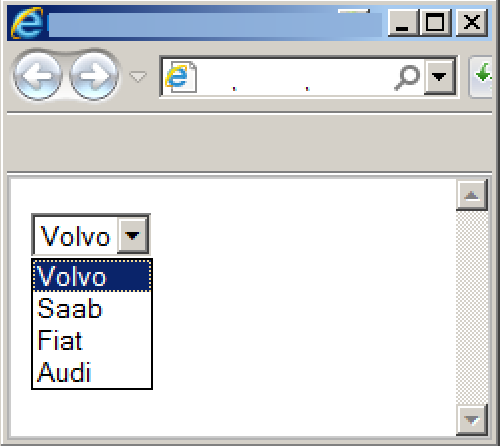
\includegraphics[scale=0.6]{./1.png}
\end{center}


\begin{latin}
\begin{lstlisting}[language=C++, caption=]
<html>
	<body>
		<select name="cars">
			<option value="volvo">Volvo</option>
			<option value="saab">Saab</option>
			<option value="fiat">Fiat</option>
			<option value="audi">Audi</option>
		</select>
	</body>
</html>
\end{lstlisting}
\end{latin}


\newpage


\begin{LTR}
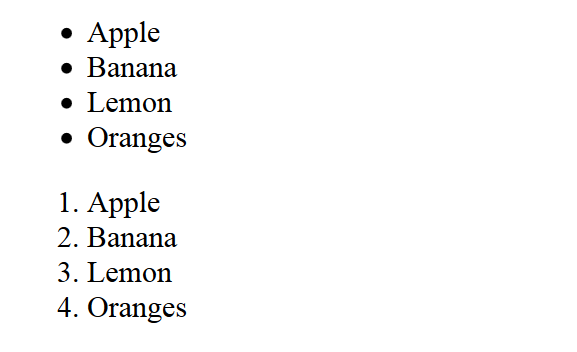
\includegraphics[scale=0.6]{./2.png}
\end{LTR}



\begin{latin}
\begin{lstlisting}[language=C++, caption=]
<html>
<body>
	<ul>
		<li>Apple</li>
		<li>Banana</li>
		<li>Lemon</li>
		<li>Oranges</li>
	</ul>
	
	<ol>
		<li>Apple</li>
		<li>Banana</li>
		<li>Lemon</li>
		<li>Oranges</li>
	</ol>
</body>
</html>
\end{lstlisting}
\end{latin}




\newpage


\begin{center}
	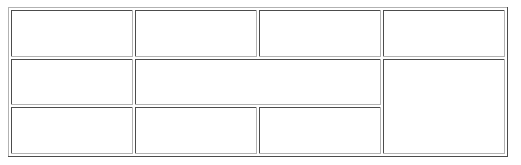
\includegraphics[scale=0.6]{./3.png}
\end{center}



\begin{latin}
\begin{lstlisting}[language=C++, caption=]
<html>
	<body>
		<table border="1" width="500" height="150">
			<tr>
				<td></td>
				<td></td>
				<td></td>
				<td></td>
			</tr>
			<tr>
				<td></td>
				<td colspan="2"></td>
				<td rowspan="2"></td>
			</tr>
			<tr>
				<td></td>
				<td></td>
				<td></td>
			</tr>
		</table>
	</body>
</html>
\end{lstlisting}
\end{latin}



\newpage


\begin{center}
	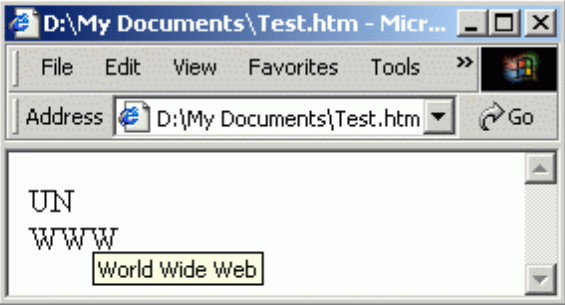
\includegraphics[scale=0.6]{./4.png}
\end{center}


\begin{latin}
\begin{lstlisting}[language=C++, caption=]
<html>
	<body>
		<abbr title="United Nations">UN</abbr>
		<br>
		<acronym title="World Wide Web " >WWW</acronym>
	</body>
</html>
\end{lstlisting}
\end{latin}



\newpage

\vspace{20pt}

\noindent
با استفاده از تگ های 
\lr{HTML}
یک فرم ثبت نمره دانشجویی ایجاد کنید که
\begin{itemize}
	\item کد دانشجویی
	\item نام درس ( با استفاده از جعبه ی پایین افتادنی )
	\item نمره ی درس
	\item دکمه ی ثبت
	\item انصراف
\end{itemize}
 باشد .
 
 \vspace{20pt}
 
\noindent
 جواب در صفحه ی بعد
 
\newpage
 
\begin{LTR}
	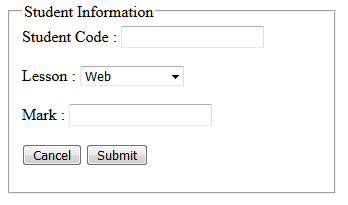
\includegraphics[scale=0.8]{./form.png}
\end{LTR}
 
 
 \begin{latin}
\begin{lstlisting}[language=C++, caption=]
<html>
	<body>
		<fieldset style="width:300">
			<legend>Student Information</legend>
			<form>
			Student Code : <input type="text" /> 
			<br /> <br />
			Lesson : 
			<select name="lesson">
				<option value="Web">Web</option>
				<option value="Programming">Programming</option>
				<option value="Database">Database</option>
				<option value="Network">Network</option>
			</select>
			<br /> <br />
			Mark : <input type="text" /> 
			<br /> <br />
			<button>Cancel</button>
			<input type="submit" value="Submit" />
			</form>
		</fieldset>
	</body>
</html>
\end{lstlisting}
\end{latin}

 


\newpage
 
 

 
\noindent
 انتخابگرهای زیر چه تفاوتی با یکدیگر دارند ؟
 
\vspace{20pt}
 
\begin{latin}
\begin{lstlisting}[language=C++, caption=]
p 
{
	background-color : yellow ;
}
\end{lstlisting}
\end{latin}



تمامی تگ های 
$<p>$
را انتخاب و رنگ پشت زمینه آنها را زرد می کند .


\vspace{60pt}


\begin{latin}
\begin{lstlisting}[language=C++, caption=]
h1 , p 
{
	background-color : yellow ;
}
\end{lstlisting}
\end{latin}







تمامی تگ های 
$<h1>$
و
$<p>$
را انتخاب و رنگ پشت زمینه آنها را زرد می کند .



\vspace{60pt}


\begin{latin}
\begin{lstlisting}[language=C++, caption=]
div p 
{
	background-color : yellow ;
}
\end{lstlisting}
\end{latin}
 
 

تمامی تگ های 
$<p>$
که در داخل تگ
$<div>$
قرار دارند را انتخاب و رنگ پشت زمینه آنها را زرد می کند .




\newpage
 
\vspace{20pt}

\noindent
با استفاده از دستورات
\lr{CSS}
ویژگی تگ پاراگراف را تغییر دهید به صورتی که 
\begin{itemize}
	\item رنگ پس زمینه زرد شود
	\item ابعاد 100 در 200 پیکسل
\end{itemize}




\begin{latin}
\begin{lstlisting}[language=C++, caption=]
p 
{
	background-color : yellow ;
	width : 100px;
	height : 200px;
}
\end{lstlisting}
\end{latin}


\end{document}